\definecolor{green}{RGB}{0,128,0}
  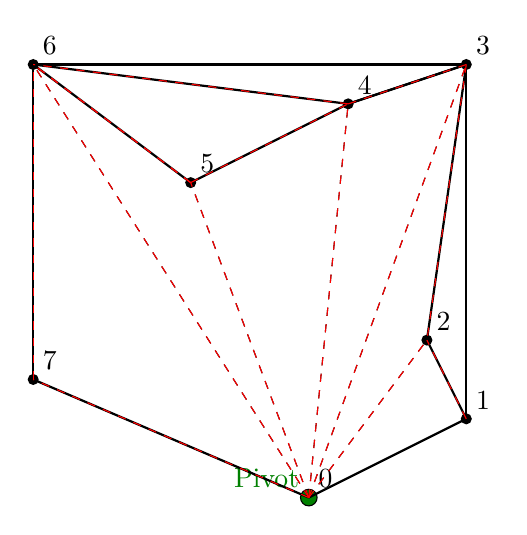
\begin{tikzpicture}
    % Define the points
    \coordinate (A) at (4,0);
    \coordinate (B) at (6,1);
    \coordinate (C) at (5.5, 2);
    \coordinate (D) at (6, 5.5);
    \coordinate (E) at (4.5, 5);
    \coordinate (F) at (2.5, 4.0);
    \coordinate (G) at (0.5, 5.5);
    \coordinate (H) at (0.5, 1.5);
    
    % Draw the points
    \foreach \point in {A,B,C,D,E,F,G,H}
      \fill (\point) circle (2pt);

    % Mark the pivot point
    \onslide<2->{
    \draw[fill=green] (A) circle (3pt);
    \node[above left, green] at (A) {Pivot};
    }

    % Draw a dashed line between the pivot and the points
    \onslide<3-4>{
        \draw[dashed] (A) -- (B);
        \draw[dashed] (A) -- (C);
        \draw[dashed] (A) -- (D);
        \draw[dashed] (A) -- (E);
        \draw[dashed] (A) -- (F);
        \draw[dashed] (A) -- (G);
        \draw[dashed] (A) -- (H);
    }
    
    % Label the points
    \onslide<4->{
        \node[above right] at (A) {0};
        \node[above right] at (B) {1};
        \node[above right] at (C) {2};
        \node[above right] at (D) {3};
        \node[above right] at (E) {4};
        \node[above right] at (F) {5};
        \node[above right] at (G) {6};
        \node[above right] at (H) {7};
        % \node[above right] at (A) {A};
        % \node[above right] at (B) {B};
        % \node[above right] at (C) {C};
        % \node[above right] at (D) {D};
        % \node[above right] at (E) {E};
        % \node[above right] at (F) {F};
        % \node[above right] at (G) {G};
        % \node[above right] at (H) {H};
    }


    \onslide<5->{
        \draw[thick] (A) -- (B);
    }

    \onslide<6-7>{
        \draw[thick] (B) -- (C);
    }

    \onslide<7>{
        \draw[thick] (C) -- (D);
    }

    \onslide<8->{
        \draw[thick] (B) -- (D);
    }

    \onslide<9-11>{
        \draw[thick] (D) -- (E);
    }
    \onslide<10-11>{
        \draw[thick] (E) -- (F);
    }

    \onslide<11>{
        \draw[thick] (F) -- (G);
    }

    \onslide<12>{
        \draw[thick] (D) -- (E);
        \draw[thick] (E) -- (G);
    }

    \onslide<13->{
        \draw[thick] (D) -- (G);
    }

    \onslide<14->{
        \draw[thick] (G) -- (H);
    }

    \onslide<15->{
        \draw[thick] (H) -- (A);
    }

    
    \onslide<6->{\draw[dashed,red] (A) -- (C);\draw[dashed,red] (B) -- (C);}
    \onslide<7->{\draw[dashed,red] (A) -- (D);\draw[dashed,red] (D) -- (C);}
    \onslide<9->{\draw[dashed,red] (A) -- (E);\draw[dashed,red] (D) -- (E);}
    \onslide<10->{\draw[dashed,red] (A) -- (F);\draw[dashed,red] (F) -- (E);}
    \onslide<11->{\draw[dashed,red] (A) -- (G);\draw[dashed,red] (F) -- (G);}
    \onslide<12->{\draw[dashed,red] (F) -- (G);\draw[dashed,red] (E) -- (G);}
    \onslide<14->{\draw[dashed,red] (A) -- (H);\draw[dashed,red] (H) -- (G);}

  \end{tikzpicture}
